\documentclass[12pt, twoside]{article}
\usepackage[letterpaper, margin=1in, headsep=0.5in]{geometry}
\usepackage[english]{babel}
\usepackage[utf8]{inputenc}
\usepackage{amsmath}
\usepackage{amsfonts}
\usepackage{amssymb}
\usepackage{tikz}
\usetikzlibrary{quotes, angles}
\usepackage{graphicx}
\usepackage{enumitem}
\usepackage{multicol}

\newif\ifmeta
\metatrue %print standards and topics tags

\title{Regents Geometry}
\author{Chris Huson}
\date{September 2020}

\usepackage{fancyhdr}
\pagestyle{fancy}
\fancyhf{}
\renewcommand{\headrulewidth}{0pt} % disable the underline of the header
\raggedbottom


\fancyhead[LE]{\thepage}
\fancyhead[RO]{\thepage \\ Name: \hspace{4cm} \,\\}
\fancyhead[LO]{BECA / Dr. Huson / Geometry 02-Midpoint+distance\\* pset ID: 31}

\begin{document}

\subsubsection*{2-8HW-Parameter-solving}
\begin{enumerate}
\item Find the area of $\triangle ABC$. The altitude $h$ of the triangle is $11 \frac{1}{3}$ centimeters and the base $AB=24$ cm.\\[0.5cm]
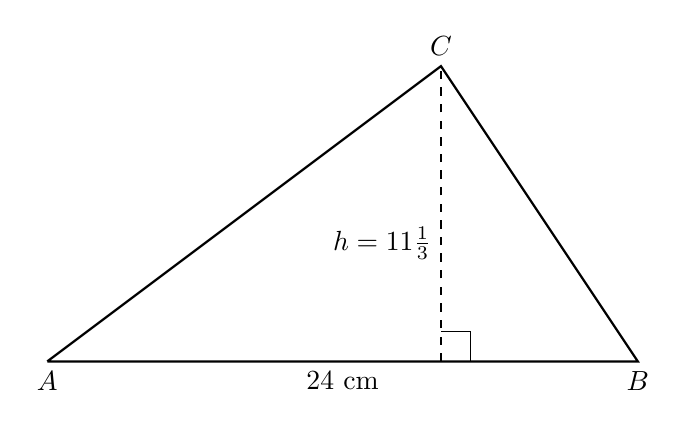
\begin{tikzpicture}[scale=1.25]
  \draw [thick]
    (2,0)node[below]{$A$}--
    (8,0)node[below]{$B$}--
    (6,3)node[above]{$C$} --(2,0);
 \draw [dashed] (6,0)--(6,3);
 \draw (6,0)++(0.3,0)--++(0,0.3)--+(-0.3,0);
 \node at (6,1.2)[left]{$h=11 \frac{1}{3}$};
 \node at (5,0)[below]{$24$ cm};
\end{tikzpicture} \vspace{1.0cm}

\item Given the rectangle $ABCD$ shown below, with $BC=6 \frac{1}{4}$. If the area of the rectangle is 100, find $AB$.
\begin{flushleft}
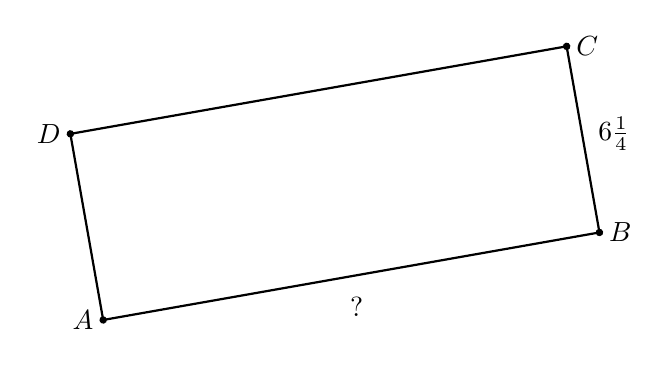
\begin{tikzpicture}[scale=0.8, rotate=10]
  \draw [-, thick] (0,0)--(8,0)--(8,3)--(0,3)--cycle;
  \draw [fill] (0,0) circle [radius=0.05] node[left]{$A$};
  \draw [fill] (8,0) circle [radius=0.05] node[right]{$B$};
  \draw [fill] (8,3) circle [radius=0.05] node[right]{$C$};
  \draw [fill] (0,3) circle [radius=0.05] node[left]{$D$};
  \node at (8.5, 1.5){$6 \frac{1}{4}$};
  \node at (4, -0.5){?};
\end{tikzpicture}
\end{flushleft}
\vspace{1.5cm}

\item Given that the area of $\triangle KLM$ is $81 \frac{1}{4}$ and the base $KL=20$. Find the altitude $h$ of the triangle.\\[0.5cm]
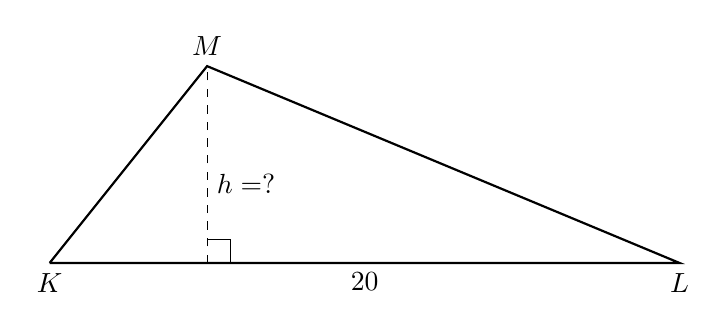
\begin{tikzpicture}[scale=1]
  \draw [thick]
    (-5,0)node[below]{$K$}--
    (3,0)node[below]{$L$}--
    (-3,2.5)node[above]{$M$} --(-5,0);
 \draw [dashed] (-3,0)--(-3,2.5);
 \draw (-3,0)++(0.3,0)--++(0,0.3)--+(-0.3,0);
 \node at (-3,1)[right]{$h=?$};
 \node at (-1,0)[below]{$20$};
\end{tikzpicture} \vspace{1.0cm}

\newpage
\item Given $\overleftrightarrow{DG}$ as shown on the number line, with $D=11$ and $G=26$. \\[15pt]
  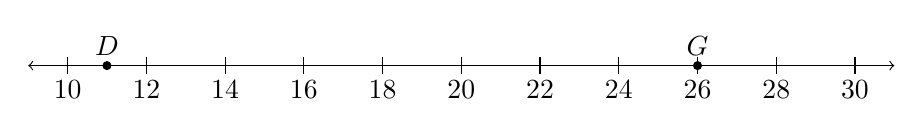
\begin{tikzpicture}[scale=0.5]
    \draw [<->] (9,0)--(31,0);
    \foreach \x in {10, 12,...,30} %2 leading for diff!=1
      \draw[shift={(\x,0)},color=black] (0pt,-6pt) -- (0pt,6pt) node[below=5pt]  {$\x$};
      \draw [fill] (11,0) circle [radius=0.1] node[above] {$D$};
      \draw [fill] (26,0) circle [radius=0.1] node[above] {$G$};
  \end{tikzpicture} \\[10pt]
  Points $E$ and $F$ trisect $\overline{DG}$. Find the values of $E$ and $F$ and mark and label them on the number line $\overleftrightarrow{DG}$. \vspace{6cm}

\item Given $\overline{PQR}$, with $PQ=\frac{1}{2} x+4$, $QR=x+3$, and $PR=2x+5$. Find ${PR}$.\\
  Complete all the steps for full credit. \smallskip
  \vspace{9cm}

\end{enumerate}
\end{document}